%% AMS-LaTeX Created with the Wolfram Language : www.wolfram.com

\documentclass{article}
\usepackage{amsmath, amssymb, graphics, setspace}

\newcommand{\mathsym}[1]{{}}
\newcommand{\unicode}[1]{{}}

\newcounter{mathematicapage}
\begin{document}

\begin{doublespace}
\noindent\(\pmb{\text{Remove}[\text{{``}Global$\grave{ }$*{''}}];}\\
\pmb{\text{Off}[\text{General}\text{::}\text{Spell1}];}\\
\pmb{\text{ClearAll}[\text{{``}Global $\grave{ }$*{''}}];}\)
\end{doublespace}

\begin{doublespace}
\noindent\(\pmb{\text{(*}\text{Factorizar} \text{el} \text{n{\' u}mero} M=15\text{*)}}\\
\pmb{M=15;}\\
\pmb{\text{(*x es el n{\' u}mero por el que se multiplicar{\' a} en el algoritmo*)}}\\
\pmb{x=\text{RandomInteger}[\{2,M-2\}]}\\
\pmb{\text{GCD}[x,M]==1}\)
\end{doublespace}

\begin{doublespace}
\noindent\(7\)
\end{doublespace}

\begin{doublespace}
\noindent\(\text{True}\)
\end{doublespace}

\begin{doublespace}
\noindent\(\pmb{\text{(*}\text{Los} |0> y |1>\text{*)}}\\
\pmb{\text{ket}_0=\{\{1\},\{0\}\};}\\
\pmb{\text{ket}_1=\{\{0\},\{1\}\};}\\
\pmb{}\\
\pmb{\text{(*El operador identidad*)}}\\
\pmb{\text{Id}=\text{IdentityMatrix}[2];}\\
\pmb{}\\
\pmb{\text{(*Las matrices de Pauli*)}}\\
\pmb{X=\text{PauliMatrix}[1];}\\
\pmb{Y=\text{PauliMatrix}[2];}\\
\pmb{Z=\text{PauliMatrix}[3];}\\
\pmb{}\\
\pmb{\text{(*La compuerta de Hadamard*)}}\\
\pmb{H=\text{HadamardMatrix}[2];}\\
\pmb{}\\
\pmb{\text{(*Los proyectores de la base computacional*)}}\\
\pmb{P_0=\text{ket}_0.\text{ConjugateTranspose}\left[\text{ket}_0\right];}\\
\pmb{P_1=\text{ket}_1.\text{ConjugateTranspose}\left[\text{ket}_1\right];}\\
\pmb{}\\
\pmb{\text{(*Operador de cambio de fase*)}}\\
\pmb{R[\phi \_]\text{:=}P_0 + e^{i \phi } P_1;}\\
\pmb{}\\
\pmb{\text{(*Compuertas condicionales*)}}\\
\pmb{\text{CNOT}=\text{KroneckerProduct}\left[P_0,\text{Id}\right]+\text{KroneckerProduct}\left[P_1,X\right];}\\
\pmb{\text{CR}[\phi \_]\text{:=}\text{KroneckerProduct}\left[P_0,\text{Id}\right]+\text{KroneckerProduct}\left[P_1,R[\phi ]\right];}\\
\pmb{\text{CR13}[\phi \_]\text{:=}\text{KroneckerProduct}\left[P_0,\text{Id},\text{Id}\right]+\text{KroneckerProduct}\left[P_1,\text{Id},R[\phi ]\right];}\\
\pmb{}\\
\pmb{\text{(*Ket general de la base computacional de dimensi{\' o}n 16*)}}\\
\pmb{\text{ket}[\text{n$\_$}]\text{:=}\text{Table}[\{n==i-1\},\{i,1,16\}]\text{/.}\{\text{True}\to 1,\text{False}\to 0\};}\\
\pmb{}\\
\pmb{\text{(*Operador de multiplicaci{\' o}n m{\' o}dulo*)}}\\
\pmb{\text{Urp}[\text{x$\_$},\text{N$\_$}]\text{:=}\text{Sum}[\text{ket}[\text{Mod}[x i,N]].\text{ConjugateTranspose}[\text{ket}[i]],\{i,0,N-1\}]+\text{Sum}[\text{ket}[i].\text{ConjugateTranspose}[\text{ket}[i]],\{i,N,15\}];}\\
\pmb{}\\
\pmb{\text{(*Matriz de densidad*)}}\\
\pmb{\rho [\psi \_]\text{:=}\psi .\text{ConjugateTranspose}[\psi ];}\\
\pmb{}\\
\pmb{\text{(*}\text{Operador} \text{para} \text{la} \text{estimaci{\' o}n} \text{de} \text{fase}: \text{Operador} \text{de} \text{multiplicaci{\'
o}n} \text{por} 7 \text{m{\' o}dulo} 15\text{*)}}\\
\pmb{U=\text{Urp}[x,M];}\\
\pmb{}\\
\pmb{\text{(*Preparando el estado inicial*)}}\\
\pmb{\text{$\psi $0}=\text{KroneckerProduct}\left[\text{ket}_0,\text{ket}_0,\text{ket}_0,\text{ket}_0\right];}\\
\pmb{\text{$\psi $0}=N[\text{KroneckerProduct}[H,H,H,H].\text{$\psi $0}];}\\
\pmb{\psi =\text{KroneckerProduct}\left[\text{ket}_0,\text{ket}_0,\text{ket}_0,\text{ket}_1\right];}\\
\pmb{}\\
\pmb{\text{$\psi $t}=N[\text{KroneckerProduct}[\text{$\psi $0},\psi ]];}\\
\pmb{}\\
\pmb{\text{(*Estimaci{\' o}n de fase*)}}\\
\pmb{\text{$\psi $t}=N\left[\left(\text{KroneckerProduct}\left[\text{Id},\text{Id},\text{Id},P_0,\text{Id},\text{Id},\text{Id},\text{Id}\right]+\text{KroneckerProduct}\left[\text{Id},\text{Id},\text{Id},P_1,U\right]\right).\text{$\psi
$t}\right];}\\
\pmb{\text{$\psi $t}=N\left[\left(\text{KroneckerProduct}\left[\text{Id},\text{Id},P_0,\text{Id},\text{Id},\text{Id},\text{Id},\text{Id}\right]+\text{KroneckerProduct}\left[\text{Id},\text{Id},P_1,\text{Id},\text{MatrixPower}[U,2]\right]\right).\text{$\psi
$t}\right];}\\
\pmb{\text{$\psi $t}=N\left[\left(\text{KroneckerProduct}\left[\text{Id},P_0,\text{Id},\text{Id},\text{Id},\text{Id},\text{Id},\text{Id}\right]+\text{KroneckerProduct}\left[\text{Id},P_1,\text{Id},\text{Id},\text{MatrixPower}\left[U,2^2\right]\right]\right).\text{$\psi
$t}\right];}\\
\pmb{\text{$\psi $t}=N\left[\left(\text{KroneckerProduct}\left[P_0,\text{Id},\text{Id},\text{Id},\text{Id},\text{Id},\text{Id},\text{Id}\right]+\text{KroneckerProduct}\left[P_1,\text{Id},\text{Id},\text{Id},\text{MatrixPower}\left[U,2^3\right]\right]\right).\text{$\psi
$t}\right];}\\
\pmb{}\\
\pmb{\text{(*}\text{QFT}^{-1}\text{*)}}\\
\pmb{\text{$\psi $t}=N\left[\text{KroneckerProduct}\left[\text{ConjugateTranspose}\left[\text{FourierMatrix}\left[2^4\right]\right],\text{Id},\text{Id},\text{Id},\text{Id}\right].\text{$\psi
$t}\right];}\\
\pmb{}\\
\pmb{\text{(*}\text{Medidas}\text{*)}}\\
\pmb{\text{For}[i=0,i<16,i\text{++},\text{sub0}=\text{Mod}[i,2];}\\
\pmb{\text{sub1}=\text{Which}[i==0,0,\text{Mod}[i,2]==0\&\&\text{sub1}==0,1,\text{Mod}[i,2]==0\&\&\text{sub1}==1,0,\text{True},\text{sub1}];}\\
\pmb{\text{sub2}=\text{Which}\left[i==0,0,\text{Mod}\left[i,2^2\right]==0\&\&\text{sub2}==0,1,\text{Mod}\left[i,2^2\right]==0\&\&\text{sub2}==1,0,\text{True},\text{sub2}\right];}\\
\pmb{\text{sub3}=\text{Which}\left[i==0,0,\text{Mod}\left[i,2^3\right]==0\&\&\text{sub3}==0,1,\text{Mod}\left[i,2^3\right]==0\&\&\text{sub3}==1,0,\text{True},\text{sub3}\right];}\\
\pmb{\text{$\psi $t}_i=N\left[\text{KroneckerProduct}\left[P_{\text{sub3}},P_{\text{sub2}},P_{\text{sub1}},P_{\text{sub0}},\text{Id},\text{Id},\text{Id},\text{Id}\right].\text{$\psi
$t}\right];}\\
\pmb{\left.\text{$\psi $t}_i=N\left[\text{ConjugateTranspose}\left[\text{$\psi $t}_i\right].\text{$\psi $t}_i\right];\right]}\\
\pmb{}\\
\pmb{\text{(*Organizar resultados de las medidas y graficar*)}}\\
\pmb{L=\text{Table}\left[\left\{i,\frac{i}{2^4},\text{$\psi $t}_i[[1,1]]\right\},\{i,0,31\}\right];}\\
\pmb{\text{ListPlot}\left[\text{Table}\left[\left\{N\left[\frac{i}{2^4}\right],\text{$\psi $t}_i[[1,1]]\right\},\{i,0,15\}\right],\text{PlotRange}\to
\text{All}\right]}\)
\end{doublespace}

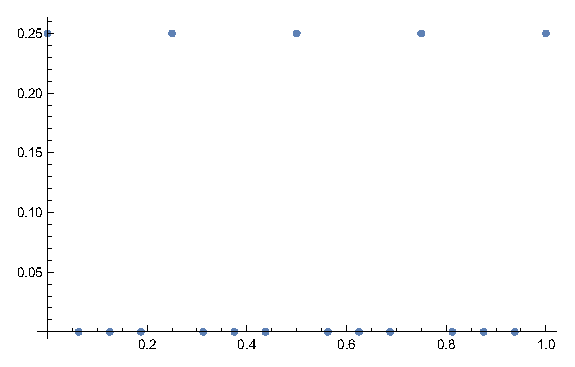
\includegraphics{Shor_gr1.eps}

\begin{doublespace}
\noindent\(\pmb{\text{(*Procesar medidas para tener la factorizaci{\' o}n*)}}\\
\pmb{\text{(*Fracciones continuas*)}}\\
\pmb{\text{L1}=\text{Table}[\{\text{Denominator}[\text{FromContinuedFraction}[\text{ContinuedFraction}[\text{Transpose}[L][[2,i]]]]],L[[i,3]]\},\{i,1,16\}];}\\
\pmb{\text{For}[i=1,i\leq \text{Dimensions}[\text{L1}][[1]],i\text{++},\text{For}[j=1,j\leq \text{Dimensions}[\text{L1}][[1]],j\text{++},\text{If}[\text{L1}[[i,1]]==\text{L1}[[j,1]]\&\&i\neq
j,\text{L1}[[i,2]]\text{+=}\text{L1}[[j,2]];}\\
\pmb{\text{L1}=\text{Drop}[\text{L1},\{j\}];]]]}\\
\pmb{\text{For}[i=1,i\leq \text{Dimensions}[\text{L1}][[1]],i\text{++},\text{If}[\text{OddQ}[\text{L1}[[i,1]]],\text{L1}=\text{Drop}[\text{L1},\{i\}];]]}\\
\pmb{\text{For}\left[i=1,i\leq \text{Dimensions}[\text{L1}][[1]],i\text{++},\text{If}\left[\text{Mod}\left[x^{\text{L1}[[i,1]]},M\right]\neq 1,\text{L1}=\text{Drop}[\text{L1},\{i\}];\right]\right]}\\
\pmb{\text{For}\left[i=1,i\leq \text{Dimensions}[\text{L1}][[1]],i\text{++},\text{If}\left[\text{GCD}\left[x^{\frac{\text{L1}[[1,1]]}{2}},M\right]==M-1,\text{L1}=\text{Drop}[\text{L1},\{i\}];\right]\right]}\\
\pmb{\text{For}\left[i=1,i\leq \text{Dimensions}[\text{L1}][[1]],i\text{++},\text{L1}[[i,2]]=\frac{\text{L1}[[i,2]]}{\text{Sum}[\text{L1}[[j,2]],\{j,1,\text{Dimensions}[\text{L1}][[1]]\}]};\right]}\\
\pmb{\text{L2}=\text{Table}\left[\left\{\text{GCD}\left[x^{\frac{\text{L1}[[i,1]]}{2}}+1,M\right],\text{L1}[[i,2]]\right\},\{i,1,\text{Dimensions}[\text{L1}][[1]]\}\right];}\\
\pmb{\text{L3}=\text{Table}\left[\left\{\text{GCD}\left[x^{\frac{\text{L1}[[i,1]]}{2}}-1,M\right],\text{L1}[[i,2]]\right\},\{i,1,\text{Dimensions}[\text{L1}][[1]]\}\right];}\)
\end{doublespace}

\begin{doublespace}
\noindent\(\pmb{\text{(*Graficar probabilidad de cada posible orden estimado*)}}\\
\pmb{\text{L1}}\\
\pmb{\text{ListPlot}[\text{L1}]}\)
\end{doublespace}

\begin{doublespace}
\noindent\(\{\{16,\text{5.200010849845537$\grave{ }$*${}^{\wedge}$-33}+0. i\},\{8,\text{6.162975822039155$\grave{ }$*${}^{\wedge}$-33}+0. i\},\{4,1.\,
+0. i\}\}\)
\end{doublespace}

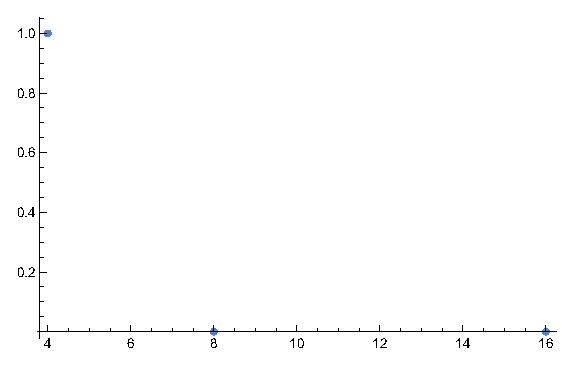
\includegraphics{Shor_gr2.eps}

\begin{doublespace}
\noindent\(\pmb{\text{(*Graficar la probabilidad de cada posible factorizaci{\' o}n hallada*)}}\\
\pmb{\text{L2}}\\
\pmb{\text{ListPlot}[\text{L2}]}\\
\pmb{\text{L3}}\\
\pmb{\text{ListPlot}[\text{L3}]}\)
\end{doublespace}

\begin{doublespace}
\noindent\(\{\{1,\text{5.200010849845537$\grave{ }$*${}^{\wedge}$-33}+0. i\},\{1,\text{6.162975822039155$\grave{ }$*${}^{\wedge}$-33}+0. i\},\{5,1.\,
+0. i\}\}\)
\end{doublespace}

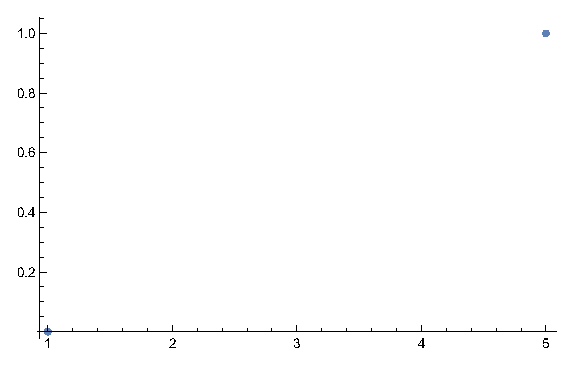
\includegraphics{Shor_gr3.eps}

\begin{doublespace}
\noindent\(\{\{15,\text{5.200010849845537$\grave{ }$*${}^{\wedge}$-33}+0. i\},\{15,\text{6.162975822039155$\grave{ }$*${}^{\wedge}$-33}+0. i\},\{3,1.\,
+0. i\}\}\)
\end{doublespace}

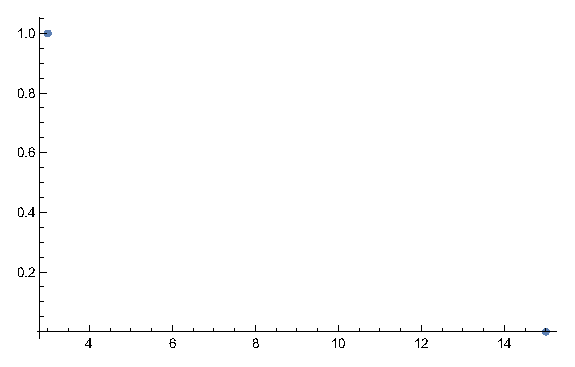
\includegraphics{Shor_gr4.eps}

\end{document}
